\documentclass[12pt]{article}
\usepackage[margin=1in]{geometry}
\usepackage{hyperref}
\usepackage{subcaption}
\usepackage{graphicx}
\usepackage[toc,page]{appendix}
\usepackage{scrextend}
\usepackage{pgfplots}
\usepackage{listings}

\setlength\parskip{5mm}
\widowpenalty10000
\clubpenalty10000
\setlength\parindent{0pt}

%\linespread{2}

\lstset{ %
  backgroundcolor=\color{white},   % choose the background color; you must add \usepackage{color} or \usepackage{xcolor}
  breakatwhitespace=false,         % sets if automatic breaks should only happen at whitespace
  breaklines=true,                 % sets automatic line breaking
  captionpos=b,                    % sets the caption-position to bottom
  escapeinside=\`\`,          % if you want to add LaTeX within your code
  extendedchars=true,              % lets you use non-ASCII characters; for 8-bits encodings only, does not work with UTF-8
  frame=single,	                   % adds a frame around the code
  keepspaces=true,                 % keeps spaces in text, useful for keeping indentation of code (possibly needs columns=flexible)
  keywordstyle=\color{blue},       % keyword style
  language=Octave,                 % the language of the code
  numbers=left,                    % where to put the line-numbers; possible values are (none, left, right)
  numbersep=5pt,                   % how far the line-numbers are from the code
  rulecolor=\color{black},         % if not set, the frame-color may be changed on line-breaks within not-black text (e.g. comments (green here))
  showspaces=false,                % show spaces everywhere adding particular underscores; it overrides 'showstringspaces'
  showstringspaces=false,          % underline spaces within strings only
  showtabs=false,                  % show tabs within strings adding particular underscores
  stepnumber=2,                    % the step between two line-numbers. If it's 1, each line will be numbered
  tabsize=2,	                   % sets default tabsize to 2 spaces
  title=\lstname                   % show the filename of files included with \lstinputlisting; also try caption instead of title
}







\title{Solving Boundary Value Problems Efficiently on Modern Computers}
\author{Daniel Bittman}



\begin{document}

\tableofcontents
\listoffigures

\section{Introduction}

Boundary Value problems history and motivation

Types of boundaries

\section{Methods}

% defines: written in C, engine, frontend
% requires: Why is C important?
The solving program is written in C\footnote{Specifically the 2011 revision to the C programming language. This means that a new enough
C compiler, one which supports C11, is needed in order to compile the program.} in order to leverage the full performance of modern computers and is implemented
as a shared library (on \textsc{unix}) such that it can be linked with another program which sets up the initial conditions
before calling the solving function. The C code that does the solving is hereby refered to as the engine, while any code
that interfaces with the engine and provides a usable user interface is referred to as the frontend.

% requires: discreet grid, boundary conditions
% defines: E config file
I have written an example frontend in Python, which is capable to parsing a configuration file which describes the
values of $f$, the initial boundary conditions, the grid size, and a number of other details about a given desired
setup (hereby collectively reffered to as a configuration). I have written several example configurations which I have used to
confirm the correctness of the solving program. For a more detailed technical description of the implementation, see Appendix~\ref{app:des}.









\subsection{Configurations and Mapping to Electrostatics}

% defines: example config file,  initial values <-> f,
% require: dirichlet, 
These configuration files are designed to be easy to write. An example configuration file is,
\begin{addmargin}[4em]{2em}
\begin{singlespace}
\texttt{gridsize 300}\\
\texttt{dirichlet 1,1 1,grid.len = math.sin(y * math.pi / grid.len)}\\
\texttt{cell 10,10 initial -100}
\end{singlespace}
\end{addmargin}
The first line sets up a grid of size 300 by 300. The second line specifies that a Dirichlet boundary condition exists
from cell $(1, 1)$ to $(1, 300)$ which takes on a value given by the expression at the end of that line. Any valid python
expression may be put here, allowing access to complex mathematical expressions. Additionally, the start and end points
do not have to define a line on a single axis, the program will do a linear interpolation to create a straight line from
	the start point to the end point.
The third line sets the initial value of
the cell $(10, 10)$ to a value of $-100$. This is the command used to define $f_{i,j}$ in equation~\ref{eq:poisson}.
An arbitrary number of these statements may be made inside a configuration file, allowing one to specify the value of
$f$ everywhere if need be, or create Dirichlet boundary conditions of arbitrary shapes.

% defines: mapping to electrostatics
The available commands for a configuration file map to various initial and boundary conditions for an electrostatics problem
in a straight forward way: the command to specifiy a Dirichlet boundary condition is like creating a boundary of fixed potential.
The command to specify the initial value of cells is like specifying an initial charge distribution inside the region.












\subsection{Verifying Correctness}

% defines: sinx potential
The clearest way to verify that the solver is working correctly is to test it out on a number of different configurations
for which the correct solution is known. My first choice here was a simple electrostatics problem straight out of a textbook\cite{griffiths}:
\begin{addmargin}[2em]{2em}% 1em left, 2em right
	Consider a square region with the bottom left corner at the origin with each side of length $L$. Let the potential
	along each side of the region be fixed at 0, except for the bottom side, which has a potential $V(x) = V_0 \sin(x \pi / L)$.
	What is the potential $V$ inside the region?
\end{addmargin}
This problem describes solving Laplace's equation (which is Poisson's equation with $f=0$), given some initial boundary conditions (hereafter referred to as ``the $\sin(x)$ potential'').
It can be solved analytically using a standard separation of variables trick\cite{boas}. Assume
$$\phi = X(x) Y(y),$$
then
$$X''(x)/X(x) = -Y''(y)/Y(y) = -\lambda,$$
and by applying the boundary conditions and using several commonly used mathematical physics techniques, one comes to the solution\cite{griffiths}
$$V(x,y) = \frac{\sinh(y \pi / L)}{\sinh(\pi / L)} \sin(x \pi / L).$$

In order to compare the result of my program with the analytical solution, I added a feature to the Python frontend
to accept a pre-made file containing a precalculated grid of the correct output by using the analytic solution. The
frontend then reads this file and compares it to the result of the solver.

Since there is now a problem which has an analytical solution, I was able to use that to describe a metric for
correctness of the simulation. I wrote a Python script that generated a 2-D grid of values based on the analytical
solution above and had it write this data structure out to disk. When the solver program was given this ``correct''
file, it would then perform a root-mean-square error calculation,
$$e_{RMS} = \sqrt{\left(\frac{\sum_{i=0}^{n} \sum_{j=0}^{n} (u_{i,j} - c_{i,j})^2}{n^2}\right)}$$
where $n$ is the length of one side of the grid, $u_{i,j}$ is the value of the calculated result at cell $(i,j)$, and
$c_{i, j}$ is the value of the analytical result at cell $(i, j)$.



% define: how to halt
However, this does not help define a way for the algorithm to determine when to halt. We cannot use an analytic solution
to determine if the simulation is close enough to a solution for every configuration we could solve for. Firstly, there
would be no point to doing this as it would imply that we already had the solution, and we will not always have the
solution to an arbitrary problem. Secondly, comparing the computed solution to a verified solution on each iteration would
be very slow. Because of this, another method for determining when the simulation has converged is required.

The method I chose was to have the simulation keep track of a sum of squares while calculating an iteration. For each cell
that it updates, it determines how much the cell's value changes. The simulation then sum the squares of all of these values
and, at the end of each iteration, it divides this sum by the number of cells in the grid and compares that to a configurable threshold.
If the scaled sum is lower than the threshold, it stops the simulation and returns. This allows the user to define a quality for
the simulation by changing the threshold value.









\subsection{Potential From Electric Dipole}
Another correctness check is a simulation of an electric dipole, since the electric potential from an electric dipole is well understood.
If two equal and opposite charges are separated on an axis by distance $d$, then at a point $p$ far away, the
potential is,
$$V = C\left(\frac{1}{r_0} - \frac{1}{r_1}\right),$$
where $r_0$ and $r_1$ are the distances from each charge, and $C$ is a constant. With some rearranging,
$$V = C\left(\frac{r_0 - r_1}{r_0 r_1}\right) = \frac{C d \cos(\theta)}{r^2},$$
where $r$ is the distance from the center of charge to the point, and $\theta$ is the angle that the line from the
center of charge forms with the axis that the dipole is on\cite{griffiths}. The potential from an electric dipole thus falls off as $1/r^2$,
which should be reflected in the solution given by the program if it is given a configuration describing a dipole.

If the solving program is correct, then if two charges are placed near each other, the numerically calculated potential
should display this $1/r^2$ behavior. I wrote such a configuration and had the frontend output the potential at points
increasing in distance from the center of the dipole, allowing me to fit the data to a $1/r^2$ curve using gnuplot\cite{gnuplot}.














\subsection{Optimization and Multithreading}
The purpose of this program is to not only be correct, but to be correct quickly. In order to achieve this, I have
tried three things in combination:
\begin{enumerate}
\item General program optimization, targeted towards 64-bit x86 machines
\item The use of the x86 SIMD instruction set
\item The use of multithreading to split up the work among CPU cores
\end{enumerate}
The first of these is pretty basic. The heavy lifting of the solver is written in C so that it can run directly on the
processor. When the program is compiled, I instruct the compiler to optimize the program to the best of its ability,
and the program is written in such a way that it can be optimized well and does not waste time doing unneccesary work.

As an example of this point, consider a 2-dimensional grid (2-D array), which must be iterated over (much like
this program does). There are two ways to do this: either iterate row-by-row, or column-by-column. The end result is
the same, and one might think the choice is arbitrary. However, when I tested the two different approaches, I found
the row-by-row approach to be around 5 times faster. This is because of caching effects and the way that the CPU
fetches data from RAM\cite{intel-1}. For a more detailed description of this, see Appendix~\ref{app:opt}.

Another example involves data structure organization. Say a program needs to store an array of objects, and each object
has data associated with it (for example, current value, previous value, error, initial state, etc). One might be tempted
to write something like in Listing~\ref{lst:aos}. The problem here is that if each object's \textsc{cur\_val} are all
calculated together (as is often the case, and is definitely the case for this solving program), then the location of
the values that need to be loaded in succession by the processor are far apart. This, again, comes down to caching
effects which are further explained in Appendix~\ref{app:opt}.

\begin{minipage}{\linewidth}
\begin{lstlisting}[frame=single,label=lst:aos,caption={Array of structures organization.}]
struct {
	double cur_val, prev_val;
	float err;
	int initial_state;
} objects[N];
\end{lstlisting}
\end{minipage}

Fortunately, this also has an easy to make change that drastically improves performance: change to structure of
arrays organization, thus reorganizing the memory layout so that related and commonly accessed-together values
appear adjacent in memory\cite{intel-opt}. This is shown in listing~\ref{lst:soa}. While it may be a less intuitive way to describe
and program a simulation, the result is significantly faster code the majority of the time.

\begin{minipage}{\linewidth}
\begin{lstlisting}[frame=single,label=lst:soa,caption={Structure of arrays organization.}]
struct {
	double cur_val[N];
	double prev_val[N];
	float err[N];
	int initial_state[N];
} objects;
\end{lstlisting}
\end{minipage}
















\subsection{SIMD Instructions}
I have also made use of the SIMD (Single Instruction Multiple Data) instruction set. These instructions are available
on modern 64-bit x86 processors\cite{intel-3a}\footnote{More instructions are added in most new releases of CPUs. There are different
SIMD instruction sets available on different processor models. I have used the sse through avx instruction sets in this
code.}. Their purpose is to enable whats known as vector processing of data on x86 machines. This provides the ability
to apply a mathematical operation to one or more arrays, and have that operation by applied to each element. For example,
I can have a 128-bit register filled with 4 values, $x=(1,2,3,4)$, and other register like it, $y=(10, 10, 11, 11)$. I can
then add them together to get $(11, 12, 14, 15)$, and this addition is issued with a single instruction. Furthermore, this
takes the same amount of time as a single addition, because the processor can do the 4 separate addition operations in
parallel\footnote{This is not the same as multithreading. The processor does these 4 separate addition operations in parallel
using 4 separate addition circuits, thus doing these operations in parallel within one core.}.

I have written in the use of SIMD instructions in the solver program in order to both reduce branches and to parallelize
the calculations required when calculating the next iteration of a given cell. I provided the ability to disable this
functionality and instead do a non-SIMD style calculation in order to get benchmarks. A requirement of the SIMD code was
that it give exactly the same result as the non-SIMD version (otherwise the implementation of the math would be incorrect).
For this reason, when talking about the results of a simulation, it does not matter if SIMD was used or not; the use
of SIMD only affects performance.

An important note is that when fully optimizing code for a machine which it knows about, \texttt{gcc} and other C compilers may choose to output
SIMD instructions in order to do computation even if the user does not do so explicitly. For this reason, in places where
I refer to the mode of the simulation as being ``non-SIMD'', what I mean is that it does not use my manual SIMD instructions
but it may still use compiler-generated SIMD instructions.

















\subsection{Multithreading}
Finally, I have added multithreading support to the solver. This is done by spitting up the grid into subregions which
are contiguous in memory, and spawning $N$ threads via the \texttt{pthreads} threading library available on \textsc{unix} systems. Each thread is then given a region to work on,
and they coordinate through shared state in order to decide when the solution has been reached. The initial implementation
showed extremely poor results with multithreading (often being drastically slowed than the single threaded version)
due to the use of atomic shared variables. It was then re-written such that the code was unsafe but much faster. This
is because each thread modifies a shared non-atomic variable that keeps track of the current total change per iteration
after that thread itself completes a number of iterations over its region. This kind of shared memory access is much faster
than coordinating the threads, but it is also technically undefined behavior in C. Fortunately, on x86, it is actually
safe, however there is potential information loss because a thread could overwrite another thread if they are trying to
update the value at the same time. A more detailed discussion of the code and why it is unsafe can be found in Appendix~\ref{app:opt}.


















\subsection{Benchmarking Performance}
Benchmarks were done by placing two calls to \texttt{gettimeofday(3)} around the core of the solver. This function has a
granularity of 1 microsecond on Linux\cite{gtod}. This code returns
both the number of iterations done and the difference between the two gettimeofday calls, which are then used to calculate
the iterations per second. In order to take into account error from unpredicatble scheduling effect from the operating system,
each benchmark was run 300 times, and the standard deviation and mean were calculated, along with 95\% confidence intervals. Several different computers were used:
computer A was an Intel Core i5-3570K with 4 cores running at 3.4GHz with 16GB of RAM. Computer B was an Intel Xeon E5620
with 4 cores with 2 threads each, running at 2.4GHz, with 24GB of RAM. Computer B did not support all of the SIMD instructions
that I used, so it was only able to benchmark the non-SIMD version of the code.



\section{Results}

All results describing the correctness of the simulation or discussing the closeness of the simulation to an analytical
result are done using the single-threaded mode. This is because this makes the result of the simulation deterministic,
and so it does not matter which machine the test was run on. For results that measure performance, the machine and options
for the simulation used will be specified. There are times when the number of threads affected the correctness of the
result.

\subsection{The $\sin(x)$ Potential}

	\begin{figure}[h]
	\centering
	\includegraphics[width=1.1\linewidth]{sin300_calc.pdf}
	\caption{Simplistic view of CPU and RAM.} 
	\label{fig:sin-result}
	\end{figure}

	\begin{figure}[h]
	\centering
	\includegraphics[width=1.1\linewidth]{sin300_exact.pdf}
	\caption{More realistic view of CPU and RAM.}
	\label{fig:sin-analytic}
	\end{figure}

Figure~\ref{fig:sin-result} shows the output of the solver program in single-threaded mode when given the $\sin(x)$ along one side
potential, plotted with the Python library matplotlib. The configuration has a grid size of 300 by 300. It matches very well with the analytical result, which
is
$$\frac{\sinh(y \pi / n)}{\sinh(\pi)} \sin(x \pi / n),$$
and is shown plotted in a similar way in figure~\ref{fig:sin-analytic}. The difference between the calculated result and the
analytical result is shown in figure~\ref{fig:sin-difference}. The values shown in the difference map are small compared
to the values in the result in all locations except the corners at the top, where the simulation does diverge somewhat, 
but never reaches values which are hugely divergence from the analytical result. Using the root-mean-square error statistic
described earlier, we have calculated that the RMS error in this simulation to be SOME NUMBER.


	\begin{figure}[h]
	\centering
	\includegraphics[width=1.1\linewidth]{sin300_diff.pdf}
	\caption{More realistic view of CPU and RAM.}
	\label{fig:sin-difference}
	\end{figure}

\subsection{Fitting to a $1/r^2$ Dipole Potential}

The dipole configuration had a grid size of 400 by 400, with all walls given a Dirichlet boundary condition
of zero. Two charges were placed near the center 10 cells apart with an arbitrary but equal and opposite charge.
The result of this simulation is shown in figure~\ref{fig:dipole-cont}, with the addition of constant-potential
contour lines. The simulation shows two opposite charges which near perfectly mirror each other. The vertical
line in the center represents a constant potential contour with a value of zero, which is expected from an
electric dipole. This is another excellent verifier that the simulation is producing correct results.

\begin{figure}[h]
	\centering
	\center
	\includegraphics[width=1.1\linewidth]{dipole_contours.pdf}
	\caption{Fitting a $1/r^2$ curve to the calculated dipole potential.} \label{fig:dipole-cont}
	\end{figure}

The potential was then measured at locations increasing in distance from the dipole in an arbitrary direction.
These data were then plotted using gnuplot, and a line of the form $y(x) = A + B / (r-r_0)^2$ was fit to the
data, which is shown in figure~\ref{fig:dipole-fit} The fit is excellent, confirming that the program had properly simulated an electric dipole. The error
bars on the data points come from the difference between successive iterations at the end of the simulation of
the dipole. They are very small, but non-zero.



	\begin{figure}[h]
	\centering
	\includegraphics[width=\linewidth]{dipole_fit.pdf}
	\caption{Fitting a $1/r^2$ curve to the calculated dipole potential.} \label{fig:dipole-fit}
	\end{figure}

The dipole is an example which lends itself to presenting another feature of the solver program. If passed the
$\texttt{-V}$ option, it will take the negative gradient of the result and plot that as a vector field. This has
the effect of plotting the electric field of the result of the simulation, which for the dipole is shown in
figure~\ref{fig:dipole-field}.

	\begin{figure}[h]
	\centering
	\includegraphics[width=0.7\linewidth]{dipole_field.pdf}
	\caption{Fitting a $1/r^2$ curve to the calculated dipole potential.} \label{fig:dipole-field}
	\end{figure}


\subsection{Performance}


Figure~\ref{fig:perf-sizes} shows the performance in iterations per second for a varying grid size for given
configuration, in this case the $\sin(x)$ along a wall potential. The performance tests were run square grids
of size 50 by 50, 300 by 300, and 1000 by 1000. For each grid size, 4 different simulation options were given:
single-threaded non-SIMD, single-threaded SIMD, multi-threaded with 4 threads non-SIMD, and multi-threaded
with 4 threads and SIMD.


\begin{figure}[h]
	\centering
	\pgfplotstableread{
		0 35 10    8 10     134 10    666 1000
		1 35 10    1461 15     134 10    666 1000
		2 132.845 1.36    127.085 3.45     297.9 23.13    222.8 26.7
	}\dataset
	\begin{tikzpicture}
    \begin{axis}[
    	xticklabels = {
    		sin50,
    	    sin300,
    	    sin1000,
    	},
        xtick=data,
        major x tick style = transparent,
        width  = 0.85*\textwidth,
        height = 8cm,
        major x tick style = transparent,
        ybar=2*\pgflinewidth,
        bar width=14pt,
        ymajorgrids = true,
        ylabel = {Run time speed (iters/sec)},
        xtick = data,
        major x tick style = {opacity=0},
        minor x tick num = 1,
        minor tick length=2ex,
        ymin=0,
        legend cell align=left,
		legend style={
	        anchor=south east,
	        column sep=1ex
	    },
        ]

\addplot[draw=black,fill=black!20, error bars/.cd, y dir=both, y explicit] table[x index=0,y index=1, y error index=2] \dataset; %Data1
\addplot[draw=black,fill=black!40, error bars/.cd, y dir=both, y explicit] table[x index=0,y index=3, y error index=4] \dataset; %Data2
\addplot[draw=black,fill=black!60, error bars/.cd, y dir=both, y explicit] table[x index=0,y index=5, y error index=6] \dataset; %Data3
\addplot[draw=black,fill=black!60, error bars/.cd, y dir=both, y explicit] table[x index=0,y index=7, y error index=8] \dataset; %Data3

	\legend{Single Threaded SIMD, Single Threaded, Multithreaded (4 threads), Multithreaded (4 threads) SIMD}
\end{axis}
\end{tikzpicture}
\caption{Different grid sizes for the $\sin(x)$ configuration, and their performance characteristics.}
\label{fig:perf-sizes}
\end{figure}

%		\addplot[ybar,fill=green,mark=none] coordinates {(0,   1513.05)};
% \addplot[ybar,fill=blue,mark=none] coordinates {(0,   1459.24)};
% \addplot[ybar,fill=red] coordinates {(0,   3174.49)};
% \addplot[ybar,fill=orange] coordinates {(0,   2354.03)};

	% \addplot[ybar,fill=green,mark=none] coordinates {(1,   1513.05)};
	% \addplot[ybar,fill=blue,mark=none] coordinates {(1,   1459.24)};
	% \addplot[ybar,fill=red] coordinates {(1,   3174.49)};
	% \addplot[ybar,fill=orange] coordinates {(1,   2354.03)};

	% \addplot[ybar,fill=green,mark=none] coordinates {(2,   1513.05)};
	% \addplot[ybar,fill=blue,mark=none] coordinates {(2,   1459.24)};
	% \addplot[ybar,fill=red] coordinates {(2,   3174.49)};
	% \addplot[ybar,fill=orange] coordinates {(2,   2354.03)};












Figure~\ref{fig:perf-numthreads} shows the performance in iterations per second of the solver when run
with the $\sin(x)$ potential with a grid size of 300 by 300. This was done on computer B, and so was done
only in non-SIMD mode. The results show a significant improvement in performance when using multiple threads
compared to the single threaded case. One may na\"{i}vely have expected the performance to scale linearly
with the number of threads; however, this would be very unlikely. As the number of threads goes up, the amount
of work that can be done in parallel would seem to scale with the number of threads, until one considers processor cache effects (specifically
cache coherency and cache size limitations). This is seen in the case of 4 threads, as it is not 4 times as fast as
the single threaded case, only about 3.2 times as fast. Increasing the number of threads quickly starts giving diminishing
returns, as the 8 threads case is now only slightly better than the 4 threads case. Recall that computer B, on which these
tests are run, has 4 cores with 2 threads each, totally 8 possible threads running in parallel. After the 8 threads case,
we start to see a drop in performance; the 16 and 32 threads case are worse than the 8 threads case. This is because
the machine cannot run more than 8 threads in parallel, so in order to have 16 threads it must rely on the scheduling
of the operating system in order to get work done. In a case of many threads, each doing heave computation and memory accesses
(as is the case here), it does not usually help to increase the number of threads beyond what the machine can handle,
as is shown here.

\begin{figure}[h]
	\centering
	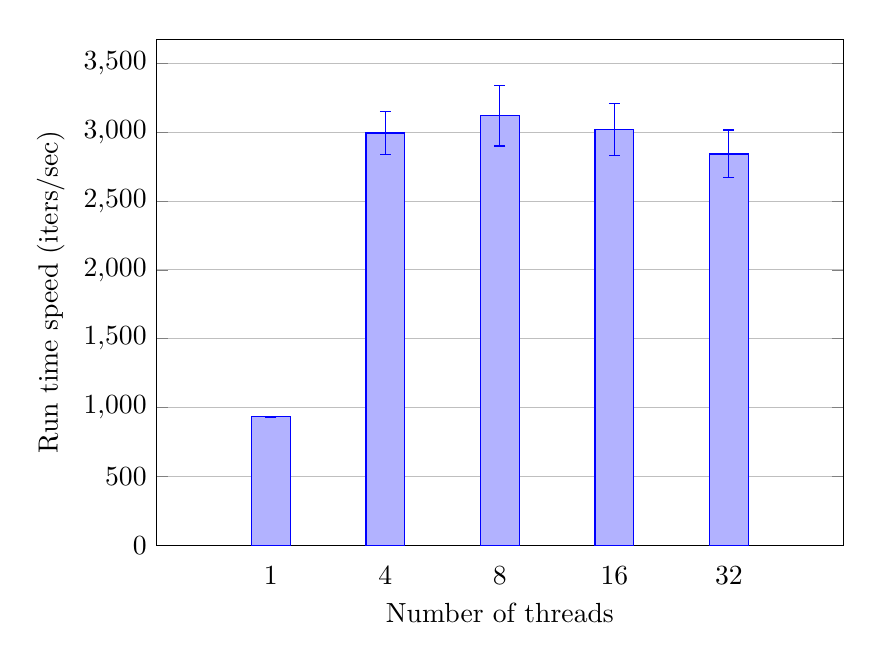
\begin{tikzpicture}
    \begin{axis}[
        xtick=data,
        symbolic x coords={1, 4, 8, 16, 32},
        major x tick style = transparent,
        width  = 0.85*\textwidth,
        height = 8cm,
        major x tick style = transparent,
        ybar=2*\pgflinewidth,
        bar width=14pt,
        ymajorgrids = true,
        ylabel = {Run time speed (iters/sec)},
        xlabel = {Number of threads},
        xtick = data,
        scaled y ticks = false,
        enlarge x limits=0.25,
        ymin=0,
        legend cell align=left,
		legend style={
	        anchor=south east,
	        column sep=1ex
	    },
        ]
            \addplot+[error bars/.cd,
                       y dir=both, y explicit]
                    coordinates {
                    (1, 933.156)  +- (3.612, 3.612)
                    (4, 2994.42)  +- (157.1, 157.1)
                    (8, 3119.1)  +- (219, 219)
                    (16, 3020.6)  +- (190, 190)
                    (32, 2842)  +- (174, 174)
                    };
\end{axis}
\end{tikzpicture}
\caption{Performance results for a varying number of threads in non-SIMD mode. These
tests were done on computer B, using the $\sin(x)$ potential with a grid size of 300 by 300.}
\label{fig:perf-numthreads}
\end{figure}



Furthermore, figure~\ref{fig:err-numthreads} shows that it is disadventagous to run the simulation with
a large number of threads. The RMS error of the simulation compared to the analytical result increases
rapidly with the number of threads. This is also reflected in the result of the simulation, which is
noticably wrong in the case of 16 or higher threads. I believe this to be the result of the way the threads
are synchronized, or more accurately, how they are not. The threads run mostly in isolation, sharing the
grid and doing operations on it without waiting for other threads to complete any of their work. This means
that if one threads runs faster than the others, it may complete a different number of iterations than the other
threads in a given amount of time. This would result in some sections of the grid recieving more iterations
than others, which could have the effect of invalidating the simulation. The alternative method would be
to synchronize the threads, and have them wait for each thread to complete a given iteration before moving on
to the next one. Indeed, this was the original design of the system, and I found it to be so slow compared to
single threaded that I changed the design around to the less accurate but much faster design that is shown here.



\begin{figure}[h]
	\centering
	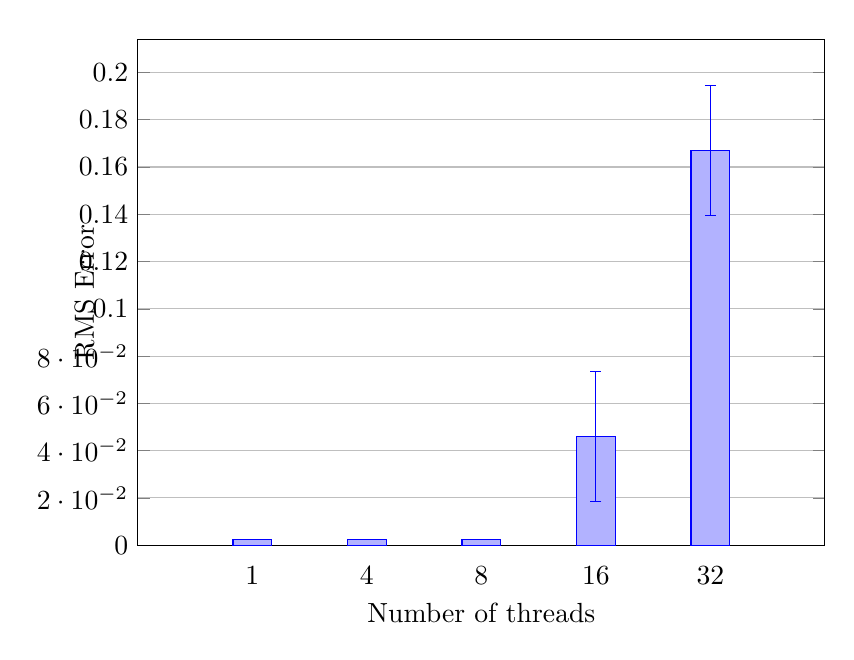
\begin{tikzpicture}
    \begin{axis}[
        xtick=data,
        symbolic x coords={1, 4, 8, 16, 32},
        major x tick style = transparent,
        width  = 0.85*\textwidth,
        height = 8cm,
        major x tick style = transparent,
        ybar=2*\pgflinewidth,
        bar width=14pt,
        ymajorgrids = true,
        ylabel = {RMS Error},
        xlabel = {Number of threads},
        xtick = data,
        y label style={at={(axis description cs:-0.05,.5)},rotate=0,anchor=south},
        enlarge x limits=0.25,
        try min ticks=10,
        ymin=0,
        legend cell align=left,
		legend style={
	        anchor=south east,
	        column sep=1ex
	    },
        ]
            \addplot+[error bars/.cd,
                       y dir=both, y explicit]
                    coordinates {
                    (1, .002544)  +- (0, 0)
                    (4, .002544)  +- (.000000027, .000000027)
                    (8, .002544)  +- (.0000000269, .0000000269)
                    (16, .046)  +- (.0274, .0274)
                    (32, .167)  +- (.0274, .0274)
                    };
\end{axis}
\end{tikzpicture}
\caption{Error results for a varying number of threads in non-SIMD mode. These
tests were done on computer B, using the $\sin(x)$ potential with a grid size of 300 by 300.}
\label{fig:err-numthreads}
\end{figure}



%32 ave: 0.166412 sq: 0.0277446 stddev: 0.00718529


\section{Conclusion}

This program correctly solves certain boundary value problems, enabling simulation
of complex electrostatics situations. It does this in an efficient manner by leveraging
proper programming languages and techniques, and by utilizing a basic understanding of modern processor
design.

\subsection{Correctness}

The most important aspect of this program is that is produces an accurate result, no
matter how fast it runs. I was able to use a problem for which I had an analytical
solution to confirm that the simulation was producing accurate results and found that
the results were of high quality for the single-threaded and low number of threads
cases. Additionally, I was able to use the solver program to accurately calculate
that the electric potential from an electric dipole drops off as $1/r^2$, further
confirming the correctness of the program.


\subsection{Performance}

Since the simulation is correct, I was able to then turn my attention towards improving
the performance without reducing the accuracy of the simulation. Most of this was easy to
do without reducing accuracy, as it was simply transforming one valid implementation of
the code into another and measuring to ensure that my new implementation did in fact
cause an improvement. Most of this was done by improving cache locality and reducing
memory accesses. I have left out a lot of this process for brevity, however an overview
of it and the concepts used can be found in Appendix~\ref{app:opt} and Appendix~\ref{app:des}.

The next significant performance gain attempt that I had made was the use of SIMD instructions.
I was hoping for a much more significant performance boost than I saw, which was rather
minuscule in reality. The rather small improvement was not surprising in the single-threaded
case because I knew that \texttt{gcc} utilizes SIMD when it can, but I did not expect to see
the manual SIMD instructions degrade the performance in the multi-threaded case. I speculate
that this is caused by my manual SIMD code being less cache friendly, which is okay in the
single-threaded case and allowed a small performance improvement, but in the multi-threaded case
the threads are all contending for limited cache space, so the additional memory usage slowed
them down.

The multi-threading actually improved the performance significantly more than I expected it to.
I had predicted that the algorithm would be cache-bound due to the large amount of memory accesses
that it makes. This often results in insignificant performance improvements (or downright performance
degradation) when adding multiple threads to a single-threaded program. Of course, the cardinal
rule of any scientific experiment (including attempting to optimize a program) is to measure and
compare results. Clearly the multi-threaded case is significantly better in performance, with a trade-off
in accuracy, which may certainly be acceptable.

\subsection{Future Work}

There is still a significant amount of optimization work that can be done on this program. A careful reading
of Intel optimization manuals would likely provide numerous ideas for how to further improve the code
of the program. The manual SIMD code could also be improved, either by utilizing more up-to-date instruction
sets or by improving the existing algorithm. The multi-threaded code could also be improved, by allowing the threads
to communicate in a limited way in order to better synchronize their work to improve the quality of the result, hopefully without
degrading the performance too drastically. An additional approach could be to use the multi-threaded case for
a few hundred iterations before switching over to the single-threaded version in order to smooth out and cleanup the
results. This would have a significant advantage for large simulations, as the multi-threaded code could get the result
most of the way before letting the single-threaded code produce an accurate result in a shorter amount of time than
if the single-threaded code run from the start.

Another significant way in which to improve the real world performance of the program could be in addition to optimizing
the speed at which the program can calculate an iteration, to reduce the number of iterations required to
converge on a solution. Indeed, this is what the use of successive over-relaxation achieves, but there may be ways
to further improve this. One such method could be to improve the initial ``guess'' of zero everywhere by dividing
the grid into a much coarser grid and running a few iterations on that before returning to the full grid and completing
the simulation as before.

\begin{center}\rule{2cm}{0.4pt}\end{center}




\clearpage
\begin{appendices}
\section{Program Usage}

Compiling the engine (the C library) requires make and gcc (or clang, though clang is untested), and can
be done by simply invoking \texttt{make}. This will also create an executable file, \texttt{solve}. This
is a script that invokes the python example frontend so that it may be used.

For more details on using the python frontend or the C backend engine, see the man pages (reproduced on the
following pages). There are several example files, including \texttt{example\_sin.txt} and \texttt{example\_dipole.txt}.
For more details on writing configurations for a desired simulation or experiment, see the man pages.

The source code also contains a directory named \texttt{tests}, which contains python code to generate verifier data
files for the \texttt{example\_sin} configuration. Finally, all of the data written on in this document are present
in the source directory, under \texttt{results}. The source code for the C library is in \texttt{engine}, and the
source code for the python example frontend is under \texttt{frontend}. The source code and git revision history
is available at \url{http://github.com/dbittman/statics-solver}.

\begin{flushleft}
	SOLVE(1)
	\hfill User Commands \hfill
	SOLVE(1)
\end{flushleft}

\begin{tabbing}
\hspace{30pt}\=\hspace{30pt}\=\kill

\textbf{NAME}\\
\> solve - Solve Discrete Poisson Equation\\
\\
\textbf{SYNOPSIS}\\
	\> \texttt{solve [-V] [-m \textit{method}] [-v \textit{verification-data}] \textit{configuration-file}}\\
	\\
\textbf{DESCRIPTION}\\
\> Solve Poisson Equation given boundary conditions on a discrete grid. Capable of\\
\> solving physics problems that reduce to a boundary value problem. Operates on the\\
\> provided configuration file, producing a 2-D array describing the calculated potential.\\
\\
\> \texttt{\textbf{-V}} \\
\> \> Produce a vector plot, where the vectors are the negative gradient of the potential.\\
\\
	\> \texttt{\textbf{-m} \textit{method}} \\
	\> \> Use method \textit{method} when solving. Current supported values are \texttt{jacobi} for\\
	\> \> Jacobi Iteration, and \texttt{sor} for Successive Over-Relaxation.\\
\\
	\> \texttt{\textbf{-v} \textit{verification-data}} \\
	\> \> Use the data file \textit{verification-data} to compare with the generated potential. The \\
	\> \> format for this file must be that of the Python library pickle serializing a 2-D array.\\
\\
\textbf{CONFIGURATION}\\
\> The configuration file format is specified by a series of commands on lines. A single line\\
\> can contain at most one command. A command must be contained within one line.\\
\> Comments begin with a \#, and comment out the rest of that line. Valid commands are\\
\> as follows, where italics indicates something to be replaced by one token:\\
\\
	\> \texttt{gridsize \textit{size}}\\
	\> \> Set the size of the grid. The grid is always a square, and this command \textbf{must}\\
	\> \> come before any other.\\
	\\
	\> \texttt{cell \textit{coords} initial \textit{value}}\\
	\> \> Specify initial value of a cell inside the grid. Analogous to a point charge.\\
	\\
	\> \texttt{dirichlet \textit{coords} \textit{coords} = \textit{value}}\\
	\> \> Specify a dirichlet boundary condition along the interpolated straight line from the\\
	\> \> first set of coordinates to the second with value \textit{value}.\\
\end{tabbing}
\begin{flushleft}
	statics-solver
	\hfill March 2016 \hfill
	SOLVE(1)
\end{flushleft}
\clearpage
\begin{flushleft}
	SOLVE(1)
	\hfill User Commands \hfill
	SOLVE(1)
\end{flushleft}

\begin{tabbing}
\hspace{30pt}\=\hspace{30pt}\=\kill
	\> \texttt{neumann \textit{coords} \textit{coords} \textit{direction} = \textit{value}}\\
	\> \> Specify a neumann boundary condition along the interpolated straight line from the\\
	\> \> first set of coordinates to the second with value \textit{value} across the boundary of the\\
	\> \> cells specified by \textit{direction}, which may be one of \texttt{left, up, right, down}.\\
	\\
	\> The values of \texttt{\textit{coords, size, direction}} must all be one token, that is,\\
	\> they may not contain any whitespace. The contents of \texttt{\textit{value}} and \texttt{\textit{coords}} are\\
	\> as follows:\\
	\\
	\> \texttt{\textit{value}} is an \texttt{expression}.\\
	\\
	\> \texttt{\textit{coords}} is an \texttt{expression} followed by a comma, followed by an \texttt{expression}.\\
	\\
	An \texttt{expression} is a valid Python expression, with access to the python math library, the\\
	current grid class, and the current position in the grid as specified by \texttt{x} and \texttt{y}. For \\
	example, \texttt{math.sin(x*math.pi/grid.len)} is a valid \texttt{expression}.\\
	\\
	\textbf{AUTHOR}\\
	\> Written by Daniel Bittman (\texttt{danielbittman1@gmail.com}). Please submit any bug\\
	\> reports to this email address.\\
	\\
	\textbf{COPYRIGHT}\\
	\> Copyright\copyright Daniel Bittman. License MIT software license. This is free software, and\\
	\> is provided with NO WARRANTY.\\
	\\

\end{tabbing}
\begin{flushleft}
	statics-solver
	\hfill March 2016 \hfill
	SOLVE(1)
\end{flushleft}


\begin{flushleft}
	SOLVER(3)
	\hfill Libraries \hfill
	SOLVER(3)
\end{flushleft}

\begin{tabbing}
\hspace{30pt}\=\hspace{30pt}\=\kill

\textbf{NAME}\\
\> solver - Library to solve Discrete Poisson Equation\\
\\
\textbf{SYNOPSIS}\\
	\> \texttt{solver.h}\\
	\> \> \texttt{SOLVE\_METHOD\_JACOBI}, \texttt{SOLVE\_METHOD\_SOR}\\
	\> \texttt{double \textbf{solve}(struct grid *grid, int method);}\\
	\> \texttt{void \textbf{init\_grid}(struct grid *grid);}\\
	\> \texttt{struct grid \{}\\
	\> \> \texttt{int len;}\\
	\> \> \texttt{int iters;}\\
	\> \> \texttt{float **values;}\\
	\> \> \texttt{float **value\_prevs;}\\
	\> \> \texttt{float **initials;}\\
	\> \> \texttt{uint8\_t **dirichlet\_presents;}\\
	\> \> \texttt{float **dirichlets;}\\
	\> \> \texttt{uint8\_t **neumann\_presents;}\\
	\> \> \texttt{float **neumanns[4];}\\
	\>\texttt{\};}\\
\\
\textbf{DESCRIPTION}\\
\> This library provides fast solving of a 2-D discrete boundary value problem using the\\
	\> Poisson equation. The full process is to define a \texttt{struct grid}, and set its \texttt{len} field.\\
	\> Then call \texttt{init\_grid} on the grid to initialize the 2-D contiguous arrays. After that,\\
	\> call \texttt{solve} and pass it the grid and a method, either \texttt{SOLVE\_METHOD\_JACOBI} or\\
	\> \texttt{SOLVE\_METHOD\_SOR}.\\
	\\
	\> The \texttt{solve} function will return when complete, returning back a value describing how\\
	\> confident it is in its result (values closer to zero are better). The \texttt{iters} field in the grid\\
	\> will have been updated to indicate how many iterations the program took. The \texttt{values}\\
	\> field points to a 2-D array of size \texttt{len} by \texttt{len} containing the solution.\\
	\\
	\textbf{AUTHOR}\\
	\> Written by Daniel Bittman (\texttt{danielbittman1@gmail.com}). Please submit any bug\\
	\> reports to this email address.\\
	\\
	\textbf{COPYRIGHT}\\
	\> Copyright\copyright Daniel Bittman. License MIT software license. This is free software, and\\
	\> is provided with NO WARRANTY.\\

\end{tabbing}
\begin{flushleft}
	statics-solver
	\hfill March 2016 \hfill
	SOLVER(3)
\end{flushleft}


\clearpage

\section{Computer Program Optimization} \label{app:opt}

\begin{addmargin}[16em]{0em}
	\begin{singlespace}
	{\footnotesize
	\textit{``Programmers waste enormous amounts of time thinking about, or worrying about, the speed of noncritical parts of their programs, and these attempts at efficiency actually have a strong negative impact when debugging and maintenance are considered. We should forget about small efficiencies, say about 97\% of the time: premature optimization is the root of all evil. Yet we should not pass up our opportunities in that critical 3\%.''}
		\begin{flushright}
		\textbf{Donald Knuth}
		\end{flushright}
	}
	\end{singlespace}
\end{addmargin}

When optimizing a program, there is an important cardinal rule to follow which at times
is easy to forget in the face of increasingly interesting and complex minor optimizations
designed to squeeze every bit of performance out of your computer. Unfortunately, due
to the complexity of modern computer hardware, it is
very difficult to predict if a given micro-optimization will actually be benificial or
not. For this reason, the most important rule when taking a working program and making it
fast is\footnote{besides \textit{don't break it}, of course. An incorrect program is worthless, no matter
how fast it is.} \textit{benchmark everything}.

The field of program optimization is huge. There is a small number of people who, for
a given platform, are really \textit{good} at optimization. There is an even smaller number
who are truly experts. I do not fit into either of these categories. For this reason, the program
that I have written here is \textit{decently} optimized. I believe that the maximum throughput
is not orders of magnitude better than what I have achieved, however, there is still a lot of work
that can be done (including a potentially significant optimization that I have neglected, and will talk
about later).

%TODO%%%%%%%%%%%%%%%%%%%%%%%%%%%%%%%%%%%%%%%%% ACTUALLY TALK ABOUT THAT ************************

\subsection{Lazy Programs Are Better}

Before taking up a sharp cutting tool and carving away a program to make it run faster, it helps to examine
what exactly is the program trying to accomplish and how. There are often multiple ways to solve a problem,
and some of them may be more efficient than others. In my case, I utilized two different methods of solving
a problem: Jacobi iteration and successive over-relaxation. One of them was significantly faster than the other
not because each iteration of the program was quicker but because it had to do less iterations. It was using a
smarter algorithm.

Computer scientists talk about algorithmic complexity using order notation. For example, given a random list
of numbers, if I want to test to see if a certain number if in the list, I need to look through the whole
list in order to check if it is there. This is an $O(n)$ operation, meaning that if the list is of size $n$, I
have to do $n$ operations to determine if the item is there or not. Data structures commonly have operations
associated with them, and those operations (such as \texttt{find}, \texttt{insert}, etc) have associated
time costs. Choosing the correct data structure for a problem is one of the first steps towards correctly
organizing a program for it to be efficient. If a program is constantly searching through a list to find
values when instead a simple hash table could be used, the program will run slowly. A program should not
do additional work when it does not need to. Only once the data structures have been properly designed
and the algorithms properly thought through should \textit{optimization} be done.

\subsection{Freebies}

There are some optimizations which can be used in high confidence and are also very easy to do.
The first, and most obvious, is to use a fast language. While writing in \texttt{C} may be a chore
compared to writing in python, the resulting code will be much faster. This is the reason behind the
organization of this program: the frontend (which has no performance requirements) is written in
python because parsing the configuration file is much easier. The backend needs to be fast, so it
is implemented in \texttt{C}.

A quick and rough experiement can easily convince you that this is true (remember how I said to
benchmark everything?). Credit to my friend Chris Milke for doing this test. Write the following
code in both python and in C: initialize a variable to zero. Then loop from zero to some large
number (we used 123,456,789), and add that iteration to the variable. After the loop, print the
variable. The resultant python program took 14.25 seconds to run on my computer, but the C code
completed \textit{instantaneously}. Why is python slower than C in general? Because python is
an interpreted language. The code that you write is read by another program and executed by
that program. In contrast, C code must be compiled into machine code. This is then run directly
on the processor, which cuts out the middle-man of the interpreter.

When using C, there are some more things that you can get for free: compiler optimizations. When
compiling a C program, the command looks something like this: \texttt{gcc -Wall -Wextra foo.c}\footnote{as an aside, you should \textbf{always} compile with -Wall and -Wextra, and eliminate all warnings from your program.
Warnings are warnings for a reason, and should rarely be ignored.}. This will
result in a compiled C program (a binary file, containing the machine code), but it will be
unoptimized. There are reasons why one may want an unoptimized binary (they are typically
easier to debug, for example), but generally when you compile your program for actual usage
you will want to optimize it. An aggressive optimization compilation command may look something
like: \texttt{gcc -Wall -Wextra -O3 -ffast-math -mavx}, as a start. The main flag here is \texttt{-O3}, which
enables almost every optimization that gcc can do.

Going back to the example from earlier, the optimized version of the C program completed instantly, but
the unoptimized version took 0.33 seconds. The unoptimized version is still 43 times faster than the
python code, but what was the optimizing compiler doing to make it so much faster with \texttt{-O3} on?
Part of optimizing is understanding why something is faster, so lets look at the assembly code. On \textsc{unix},
this can be done with the objdump command. Table \ref{table:assem-1} shows the annotated assembly from
the function \texttt{main}. If you don't know x86\_64 assembly language, you will at least notice that the
optimized version is much shorter. If you do know how to read the assembly, you'll notice that the unoptimized
version is doing almost literally what the C code says to do: set a variable to zero, and iterate from zero to
a big number, adding that iteration to the variable, and finally printing the variable. The optimized code just prints a large number -- which happens to be the result of the sum.

\begin{table}[h]
	\centering
\begin{tabular}{l | l}
	\hline
	\textbf{Unoptimized} & \textbf{Optimized}\\
	\hline
	\texttt{mov [rbp-0x10], 0x0}	&\texttt{movabs rsi,0x1b131147ee6b52} \\
	\texttt{jmp .loop\_end			}	&\texttt{mov edi,0x400594} \\
	\texttt{.loop\_top:                } &\texttt{xor eax,eax   } \\
	\texttt{mov rax, [rbp-0x10]				}	&\texttt{jmp 4003c0 <printf@plt>}\\
	\texttt{add [rbp-0x8], rax				}	&\texttt{	} \\
	\texttt{add [rbp-0x10], 0x1				}	&\texttt{ }\\	
	\texttt{.loop\_end:                       } &\texttt{} \\
	\texttt{cmp [rbp-0x10],0x75bcd14} &\texttt{} \\
	\texttt{jle loop\_top} &\texttt{} \\
	\texttt{mov rsi,[rbp-0x8]} &\texttt{} \\
	\texttt{mov edi, 0x4005b4} &\texttt{} \\
	\texttt{mov eax, 0} &\texttt{} \\
	\texttt{call 4003c0 <printf@plt>} &\texttt{} \\
\end{tabular}
	\caption{Unoptimzed and optimized assembly from the sum-a-lot-of-numbers example.}
	\label{table:assem-1}
\end{table}

This is just a simple example, but a good C compiler can drastically improve the performance of a
program. Here, it made a program that took a third of a second (which is already drastically faster than
the interpreted python version!) finish instantly.

\subsection{A Model of Processor Design}

When first learning to program in a language that does more accurately display what is going on
inside of a computer, it is helpful to have a mental model for what is going on during each
simple operation that a programmer might want to do. Since programs are sets of instructions
which define transformations on data, it is tempting to think about a model such as in figure~\ref{fig:1a},
where there is some nebulous device which follows your instructions and is connected to a large amount
of memory in which your variables and data structures live.

Unfortunately, while this is a convenient abstraction to think about programming up an application, it
is not actually what is going on\footnote{I do not claim that what I am about to describe is what is ``actually going on'' either,
but it is at least significantly less of a lie.}. A more realistic model is shown in figure~\ref{fig:1b}. There are
several key take aways from this. One of them is that RAM is \textit{really slow}. The second is that the processor
chip is aware that RAM is really slow and so it aggressively caches everything that it ever gets out of RAM. This diagram
shows the actual detailed level of caches that cores have on them, and that they have a shared cache, but most of that
complexity is not needed for a basic understanding. When one makes first steps towards optimizing a program, it is vital
to think in the more complex model, because a huge amount of time will be spent trying to optimize the program according
to how the processor actually works.

\begin{figure}[h]
\begin{subfigure}{0.4\textwidth}
\includegraphics[width=\linewidth]{ram-cpu-simple.pdf}
\caption{Simplistic view of CPU and RAM.} \label{fig:1a}
\end{subfigure}
\hfill
\begin{subfigure}{0.4\textwidth}
\includegraphics[width=\linewidth]{ram-cpu-complex.pdf}
\caption{More realistic view of CPU and RAM.} \label{fig:1b}
\end{subfigure}
\label{fig:cpu-and-ram}
\caption{View of programming that programmers like to have (a), versus the the more realistic
	and complicated view (b).}
\end{figure}

\subsubsection{Caching}

On modern processor chips, the vast majority of the silicon is used to implement a memory cache. This gives an indication
of how important it is. Think of the cache as a smaller, but much much faster memory that the processor accesses whenever
it would access RAM. If it finds the value in the cache, reading a value can take between 1 and 10's of nanoseconds. However,
if it does not find the value in the cache, it must then perform a read from memory, which can take hundreds of nanoseconds.
For scale, a single instruction very often takes less than a nanosecond to do. This means that if a program makes a lot of
memory accesses, the processor will spend a lot of time waiting and not much time calculating.

Earlier in this document, I described a phenomenon which describes how important caching is. Given a 2-D array, there are two
ways to iterate over the whole thing: line-by-line or column-by-column. On my computer, the line-by-line method was five times
faster than the alternative. This has to do with the cache, and specifically, \textit{cache lines}. When reading a value out
of memory for the first time, the processor actually reads many values, something like 64 bytes worth of data. This is fact
of the design of the hardware, and is partly because if you read a value $x$ from RAM, the processor expects you will want to
access memory that is nearby $x$ in the near future. Thus, if you iterate over an array line-by-line, when you access the
first element of a line you are actually reading in multiple elements of the array into the cache at once. When the processor
then tries to access the second element of the line, it finds that it is already in the cache, making that access much faster
than if it had not been in the cache. If you iterate over the array column-by-column, you read the first element of the line,
which loads several elements from that line into the cache, and then \textit{those values are ignored} and the first element
of the second line is read. This means that when reading the first element of the lines, each time the processor has to fetch
the value from RAM and does not get a chance to make use of the cache. By the time an entire column has been read, the cache
may be full, forcing the processor to remove old values from it. Then, when the program reads the second element of the first line,
that data no longer in the cache. This is extremely slow.

If possible, try to keep the amount of memory that the program accesses small. Try to organize the access patters such that it is
something that the processor is good at handling (like the iteration direction choice above). I have utilized these methods in my
solver program. An example for keeping memory footprint small was to reuse variables inside the grid that I knew were safe to reuse.
Additionally, I used \texttt{float}s instead of \texttt{double}s wherever possible, as this reduces memory usage as well.

\subsection{Structure of Arrays}

While I had written code that utilized the x86 SIMD extensions, this was not particularly necessary. Modern compilers are capable
of producing executables which use these instructions themselves, without the help of the programmer. Of course, a skilled programmer
may be able to write a much better version than the compiler can because they have much more context for what the program is doing,
but in general, the compiler can produce a somewhat reasonable output a lot of the time. However, one thing that it cannot do very
effectively is reorganize data access patterns into a more CPU friendly manner.

This is the reason why it is, at this point in compiler technology, worth it to restructure performance critical code to help out
the compiler and the processor as much as possible. The structure-of-arrays versus array-of-structures design options are an example
of this. As was described in section~\ref{sec:opt-mul}, there can be a significant improvement from restructuring to a structure-of-arrays
style of data organization. This is due to, for the most part, the SIMD nature of data processing. The code emitted by the compiler
is likely using SIMD style data accesses, and they are helped tremendously by being able to load a lot of the same value from different
cells at once. Because organizing the data in a SOA method places all of the values that have the same meaning for each cell next to
each other, there is a benefit seen both in the way the code is trying to access the data and in the way the processor is caching it.

\subsection{Multithreading}

Multithreading a program is a solution to performance problems that is commonly thrown out in a loose way. Multithreading something is
typically only effective when there are multiple largely independent pieces of work to be done in a system. It does not always improve
performance. This is a situation, like any other performance question, where is important to measure before and after and determine
if it is worth it.

\subsubsection{Undefined Behavior Land}

One huge problem in multithreaded programming is data synchronization. Consider a simple example, where there are four threads which
are all sharing a variable named $x$ which initially starts with a value of 4. If all threads execute the code \texttt{x++}, what are
the possible value\textbf{s} of $x$? Ideally, just 8, but that is not the case. The reason is because \texttt{x++} is really three
separate operations: 1) read $x$ into the CPU, 2) increment the value inside the CPU, and 3) write the new value to $x$ in memory.
So what happens if two threads read $x$ at the same time? They both get back 4, and the both increment it internally to 5, and write
back 5, resulting in two increment operations appearing as if only one had happened.

The answer is, $x$ could be 5, 6, 7, or 8, and there is \textit{no way to predict which one}. At least one increment will happen, and
that is all that can be known\footnote{Technically, this is not really true, as this is undefined behavior which is quite literally undefined, and
so your program could do anything from incrementing $x$ to 9 to selling your liver on the black market (though this is admittedly unlikely).}. This is an example of undefined
behaviour and is very common in multithreaded programs.

Fortunately, C11 provides a simple solution: declaring variables as \texttt{\_Atomic} (for example, \texttt{\_Atomic int x}). If $x$ in
the example above were to be declared this way, then the answer to the above problem is simply ``just 8''. The advantage is that there
is no loss of information when multiple threads operate on a single shared variable. The disadvantage is that this is slower because
it effectively ``locks'' that part of the memory and prevents other operations from occuring until one completes. This is supported
in hardware for integer types, but not floating point types. This makes atomic floating point variables particularly slow because they
need extra locking, and therefore extra memory accesses and CPU time for every access.

This was the problem I ran into when designing the multithreading in the solver application. There was a shared floating point value
to keep track of how much the simulation had changed after each iteration. This ended up being slower than the single threaded case.
By minimizing the shared state between threads and limiting the communication of floating point values between threads as much pos
possible, there was a huge performance improvement.

\subsubsection{More Threads Means More Data}

An additional concern with multiple threads is that you can run out of cache space more easily. Now, instead of sequentially operating
on some block of data (because sequential data access is fast, so that is what you would do, of course), there are multiple threads
working on different parts of memory at the same time. This means they are fighting over cache space. It is entirely possible for
adding threads to make something \textit{slower}, because of this contention. Again, the key comes down to measuring. It is hard to
know ahead of time what will help and what will not. Multithreading only makes things worse, since now the program can be run in a
non-deterministic manner: sometimes some threads will be slower, sometimes they will be faster. This makes it even harder to predict,
and more complicated to measure.

\subsection{Branch Reduction}

In programming, any statement in the language which will cause the flow of execution of the code to change based on a condition
is called a branch. This includes if statements, while loops, etc. Many times these cannot be avoided, but there are also
times when the code can be restructured in a way to reduce their number. This can be useful, because branches are often slow.
This is partially because of caching (instructions for the CPU are cached as well as data, so if it suddenly jumps far away due
to a branch, it has to load instructions from memory, which is slower). The real reason that branches are slow has to do with
pipelining in the CPU, which I will not go into here. The summary is that reducing branches is good, and organizing the required
branches in a simple way will probably be good enough for the processor to optimize them reasonably well.

\subsection{Concluding Remarks}

The most important idea when optimizing is to keep in mind that you may be wrong, so measure everything to ensure that the optimization
is actually an optimization. Secondly, a highly optimized but slow algorithm will still be slow for large enough inputs. Fast processors
do not beat order notation, and searching a hash table for a value ($O(1)$) is \textit{extremely likely} to be faster than looking it up
in an array ($O(n)$). Thirdly, make sure that there is not hidden cost in using a data structure, avoid repeated work that does not need to be repeated,
and be aware of some basic reasonably fast algorithms (sorting, for example). Fourth, use a programming language which compiles to direct processor
instructions (C, C++, among others), and use the optimization options for the language. Fifth, organize the program's data so that accessing it is
typically sequential, and try to design the layout of data such that it is easy for the compiler and the processor to optimize. Sixth, multithreading
can help, but it can also be tricky to get right. Finally, work on reducing memory footprint, branches, code complexity, and complicated slow
math if possible.

But, of course, programs should be written for correctness and clarity first, even if this means sacrificing some performance early on. However,
there is a limit to this. Faster algorithms should be used, and we should try hard not miss Donald Knuth's 3\%, as long as we remember to measure
what we have done.


\section{Program Implementation}
\label{app:des}

\end{appendices}
\end{document}

